\chapter{Nulpunktsjustering}

\section{Vejledning til nulpunktsjustering}
Her findes vejledning til korrekt indstilling af tryktransducer ved henholdsvis nulpunktsjustering og måling.

\subsection{Korrekt indstilling ved nulpunktsjustering}
\vspace{0.5 cm}
Hanen på tryktransduceren indstilles til atmosfærisk tryk ved at sørge for at der både er en pil, der har forbindelse til luften samt en pil, der har forbindelse til transduceren. Se billede nedenfor: 
\vspace{0.5 cm}
	\begin{figure}[h!]
	\centering
	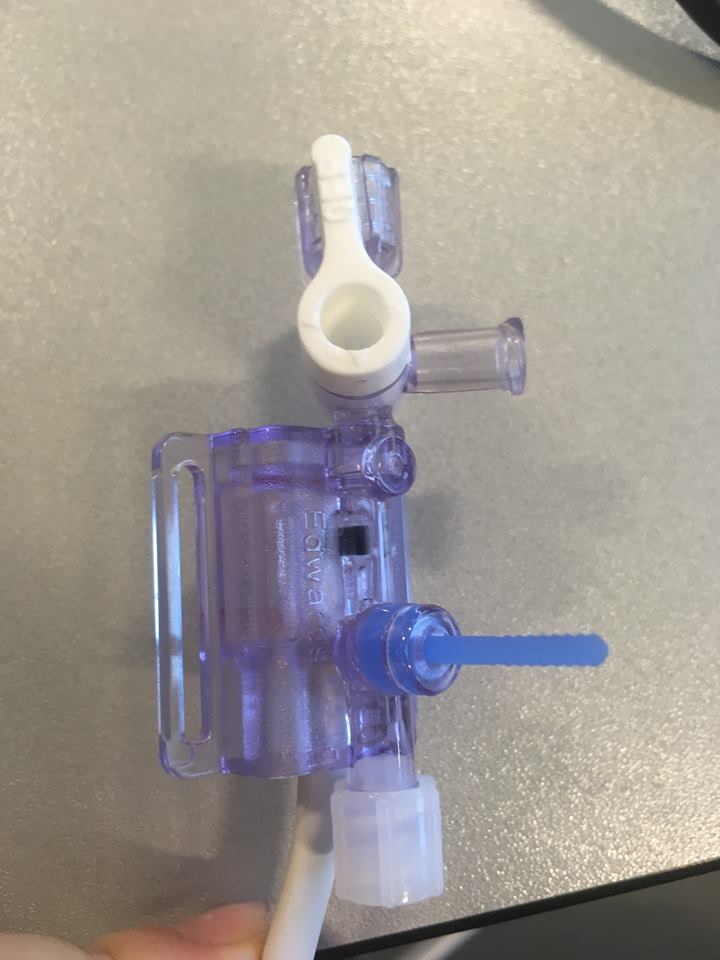
\includegraphics[width=0.3\linewidth]{Nulpunktsjustering/Nulpunktsjustering}
	\label{fig:nulpunktsjustering}
	\caption{Indstilling af hanen til nulpunktsjustering}
\end{figure}
\subsection{Korrekt indstilling ved måling}
\vspace{0.5 cm}
Hanen på tryktransduceren indstilles til måling ved at sørge for at der både er en pil, der har forbindelse til det tryk, der skal måles (Eks. fra vandsøjlen) og en pil, der har forbindelse til transduceren. Se billede nedenfor: 

\clearpage

	\begin{figure}[h!]
	\centering
	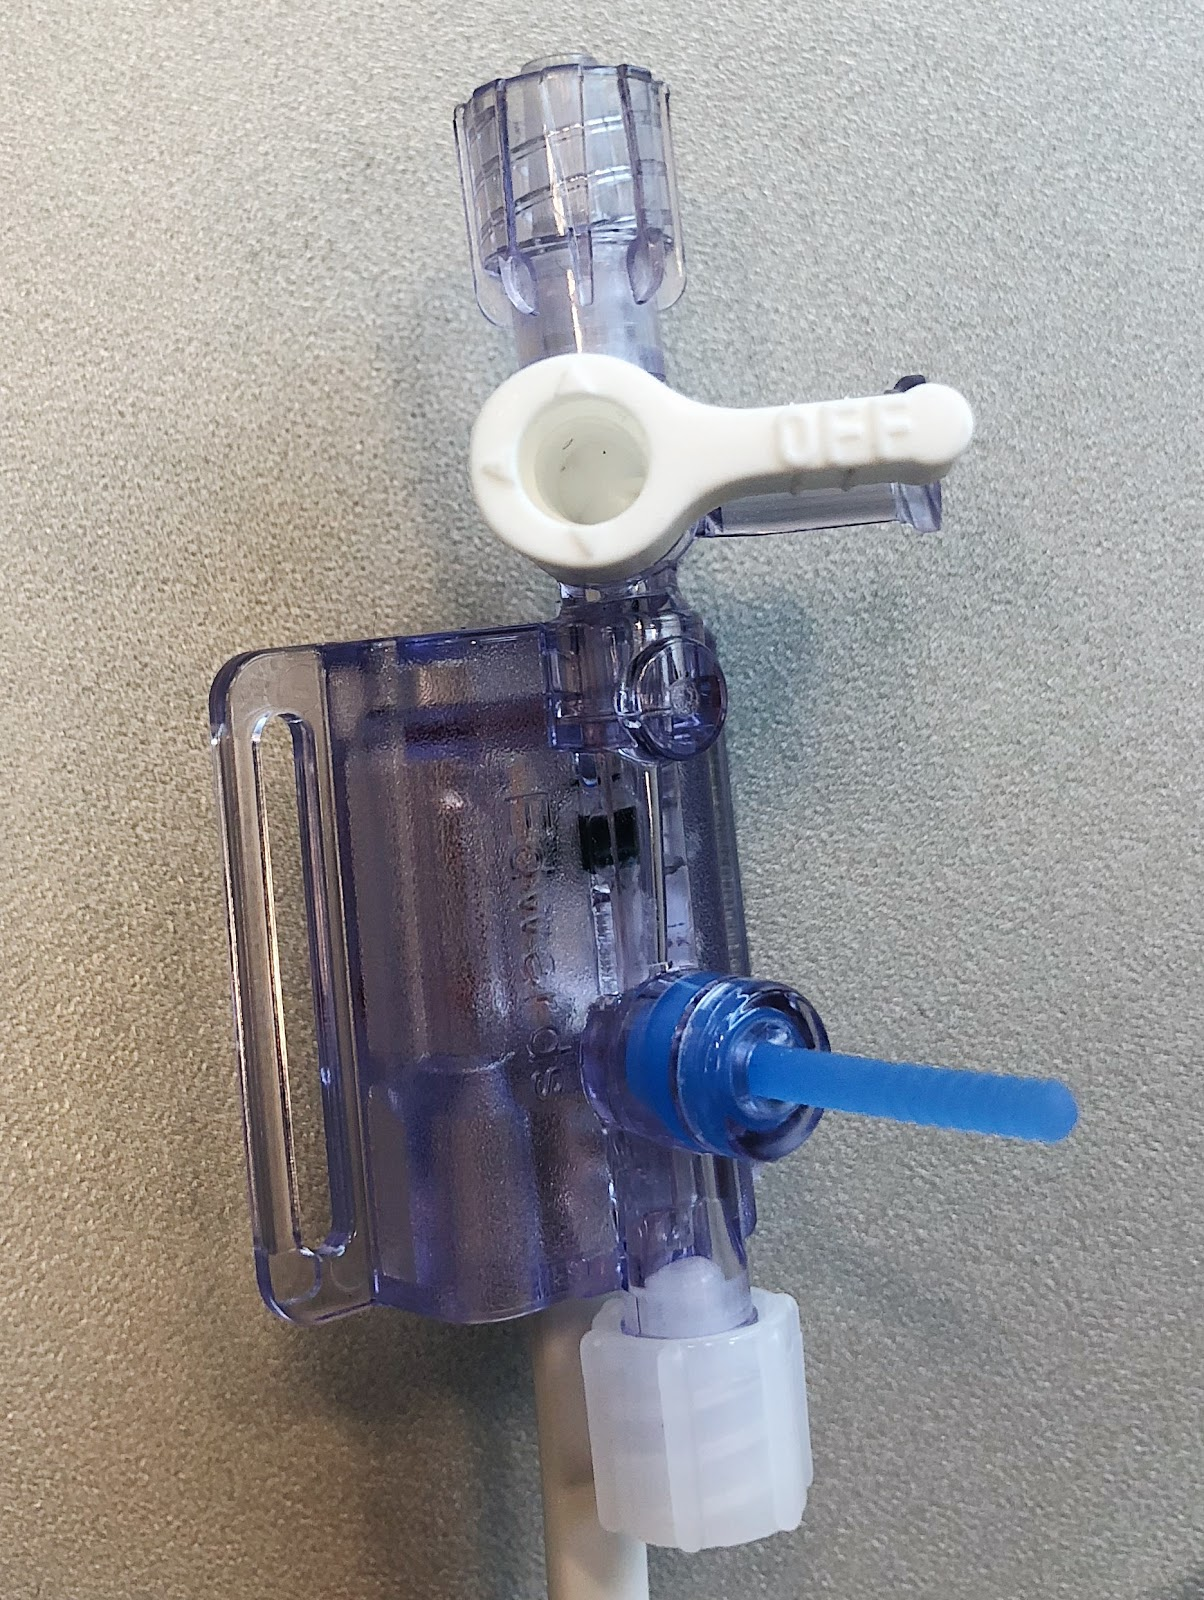
\includegraphics[width=0.3\linewidth]{Nulpunktsjustering/Maaling}
	\label{fig:maaling}
	\caption{Indstilling af hanen til måling}
\end{figure}
